\documentclass{beamer}
\usepackage{graphics}
\usepackage{epsfig}
\usepackage{multicol}
\usepackage{pifont}
\setbeamertemplate{navigation symbols}{}
\newcommand{\RR}{\ensuremath{\mathbb{R}}}
\newcommand{\NN}{\ensuremath{\mathbb{N}}}
\newcommand{\QQ}{\ensuremath{\mathbb{Q}}}
\newcommand{\CC}{\ensuremath{\mathbb{C}}}
\newcommand{\ZZ}{\ensuremath{\mathbb{Z}}}
\newcommand{\TT}{\ensuremath{\mathbb{T}}}
\newcommand{\HH}{\ensuremath{\mathbb{H}}}
\DeclareMathOperator{\Min}{Min}
\DeclareMathOperator{\Dom}{Dom}
\DeclareMathOperator{\vol}{vol}
\DeclareMathOperator{\Aut}{Aut}
\DeclareMathOperator{\Stab}{Stab}
\DeclareMathOperator{\Sym}{Sym}
\DeclareMathOperator{\Grp}{Grp}
\DeclareMathOperator{\HYP}{HYP}
\DeclareMathOperator{\CUT}{CUT}
\DeclareMathOperator{\GL}{GL}
\DeclareMathOperator{\AGL}{AGL}
\DeclareMathOperator{\Id}{Id}
\DeclareMathOperator{\mint}{min}
\DeclareMathOperator{\vertt}{vert}
\DeclareMathOperator{\conv}{conv}
\DeclareMathOperator{\rank}{rank}

\def\QuotS#1#2{\leavevmode\kern-.0em\raise.2ex\hbox{$#1$}\kern-.1em/\kern-.1em\lower.25ex\hbox{$#2$}}

\begin{document}
\title{Coupling of Geophysical Models}
\author{
\textcolor{red}{\large Mathieu Dutour Sikiri\'c},
\textcolor{red}{\large Aron Roland}, 
\textcolor{red}{\large Luigi Cavaleri},
\textcolor{red}{\large Luciana Bertotti},
\textcolor{red}{\large Lucio Torrisi}
}



\date{\today} 
\frame{\titlepage} 


\frame{
  \frametitle{Geophysical models and their coupling}

\begin{itemize}
\item The different kind of models that will be considered in this presentation are:
\begin{itemize}
\item Atmospheric models
\item Circulation models
\item Wave models
\end{itemize}
\item The parallelization of the models considered is based on {\bf MPI}.
\item The partitioning is always on geographical space. Significant exception is WaveWatchIII and maybe this will change.
\item What we will consider here is how to couple the models. We consider:
\begin{itemize}
\item {\tt ROMS} + {\tt WWM}
\item {\tt COSMO} + {\tt WAM}
\end{itemize}
\item The model grids can be structured or unstructured.
\item We designed out own library {\tt PGMCL} for easy coupling of geophysical models.
\end{itemize}
}




%\frame{
%  \frametitle{Model coupling library, {\tt PGMCL} }
%\begin{itemize}
%\item The exchange between coupled models requires the sending of data between them.
%\item A priori the grids are different, the model nature may be different (Structure/Unstructured grids) and s%o interpolation is needed between the models.
%\item There are several existing libraries {\tt MCT}, {\tt OASIS}, {\tt PALM}, etc but when considering them, they appear all relatively complicated.
%\item We considered {\tt MCT} and it appeared to be impossible to achieve the goals that we wanted (optimal exchanges, interpolation, performance, etc.).
%\item Henceforth, we designed our own library {\tt PGMCL} (Parallel Geophysical Model Coupling Library) for coupling models.
%\item After declarations, the commands become as simple as
%\begin{center}
%{\tt CALL MPI\_INTERP\_SEND(TheArr\_WAVtoOCN, Hwave)}\\
%{\tt CALL MPI\_INTERP\_RECV(TheArr\_WAVtoOCN, Hwave)}
%\end{center}
%\end{itemize}
%}







\frame{
\begin{center}
\begin{tabular*}{7cm}{c}
\\[-0.5cm]
{\Huge \textcolor{blue}{I. }\textcolor{red}{Coupling}}\\[4mm]
{\Huge \textcolor{red}{of circulation}}\\[4mm]
{\Huge \textcolor{red}{and wave models}}
\end{tabular*}
\end{center}
}




\frame{
  \frametitle{Wave coupling}

\begin{itemize}
\item Wave models use surface currents for the advection of wave energy and
the free surface enters into the dispersion relation.
\item On the other hand oceanic model can use wave information to:
\begin{itemize}
\item Compute the Stokes drift (current induced by waves, a nonlinear effect).
\item Compute the wave radiation pressure term in the primitive equation (Ardhuin formulation is prefered)
\item Improve the computation of the surface stress, turbulence.
\item Be used in sediment transport models.
\end{itemize}
\item Thus it makes sense to have oceanic and wave models coupled both ways. We chose to work with the {\tt ROMS} model (a finite difference model) and the {\tt WWM} model (a finite element model by Aron Roland).
\end{itemize}
\begin{center}
\resizebox{4cm}{!}{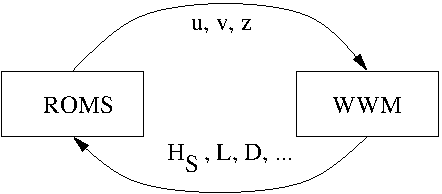
\includegraphics{FIG_wave/Model_Coupling.pdf}}\par
\end{center}
}





%\frame{
%  \frametitle{Numerics of the coupling}
%\begin{itemize}
%\item The mathematical expressions occurring in wave coupling theories are dangerous expressions like:
%\begin{equation*}
%\frac{\cosh(2k (z+h))}{\sinh(2k (h+\xi))}
%\end{equation*}
%\item This kind of function is very singular. Their large values are concentrated on the surface. On the other hand it satisfies a specific integral property:
%\begin{equation*}
%\frac{1}{h+\xi} \int_{-h}^{\xi} \frac{\cosh(2k (z+h))}{\sinh(2k (h+\xi))} dz=\frac{1}{2k(h+\xi)}
%\end{equation*}
%which has to be reproduced in the model.
%\item The solution that we choose is for every vertical cell of the model, to compute explicitly the integral and put the average value at the relevant point.
%\item We also use a $k_{eff} = \frac{1}{D} \min(300, k(h+\xi))$.
%\end{itemize}
%}










\frame{
  \frametitle{Bora event I}
\begin{center}
\begin{minipage}{5.3cm}
\centering
\resizebox{5.5cm}{!}{\includegraphics{NCLpictures_buoy/DoNCL_BoraTime/TheWindB.eps}}\par
\end{minipage}
\begin{minipage}{5.3cm}
\centering
\resizebox{5.5cm}{!}{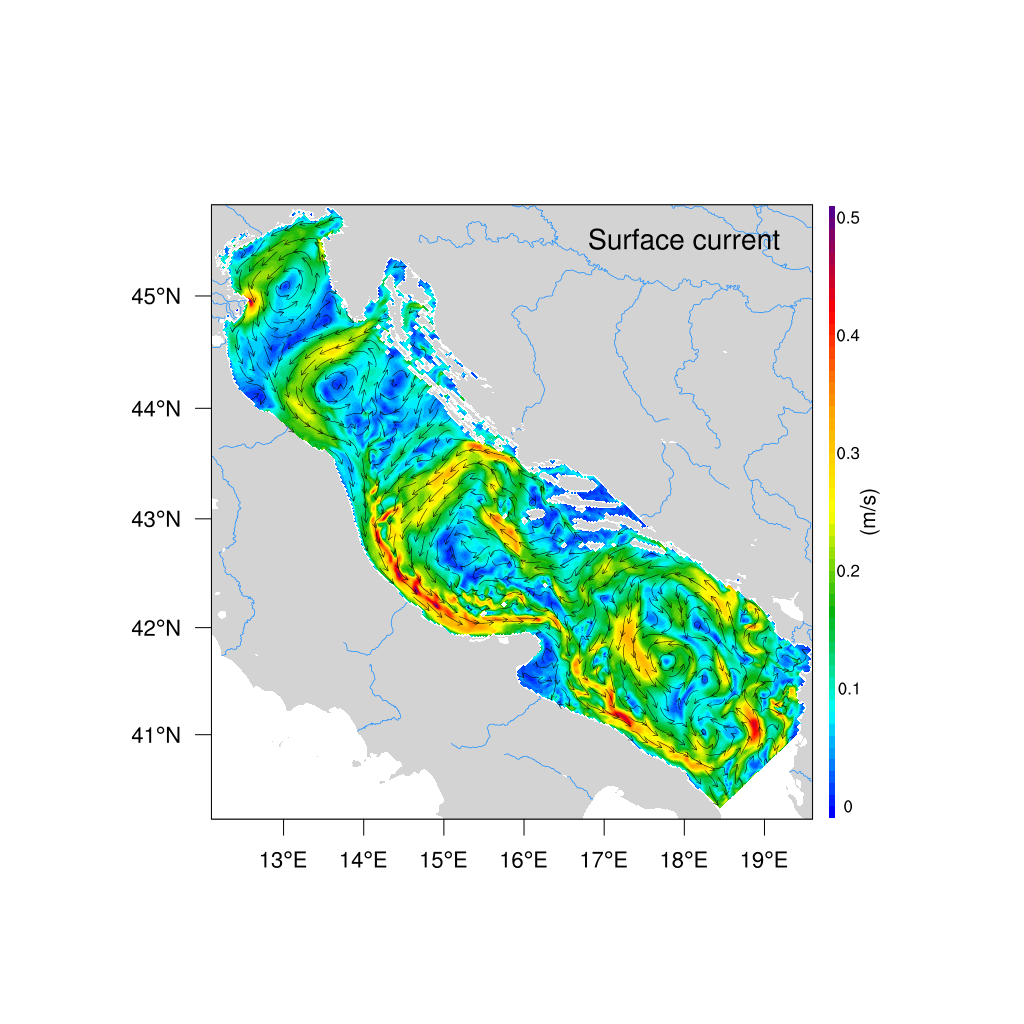
\includegraphics{NCLpictures_buoy/DoNCL_BoraTime/TheCurrentB.eps}}\par
\end{minipage}
\end{center}

\begin{itemize}
\item Wind speed and surface current at 2007-11-17 06:00:00 during a bora event.
\item The bora jets induce a multiple gyre structure on surface currents.
\end{itemize}

}




\frame{
  \frametitle{Bora event II}
\begin{center}
\begin{minipage}{5.3cm}
\centering
\resizebox{5.5cm}{!}{\includegraphics{NCLpictures_buoy/DoNCL_BoraTime/HwaveB.eps}}\par
\end{minipage}
\begin{minipage}{5.3cm}
\centering
\resizebox{5.5cm}{!}{\includegraphics{NCLpictures_buoy/DoNCL_BoraTime/DiffHwaveB.eps}}\par
\end{minipage}
\end{center}

\begin{itemize}
\item Coupling led to a decrease of $H_s$ in the bora jet and an increase outside of the jet due to opposing currents.
\end{itemize}
Work done in collaboration with M. Kuzmi\'c (IRB), I. Janekovi\'c (IRB), I. Toma\u zi\'c (ESA) and A. Roland (TU Darmstadt)
}







\frame{
\begin{center}
\begin{tabular*}{7cm}{c}
\\[-0.5cm]
{\Huge \textcolor{blue}{II. }\textcolor{red}{Coupling}}\\[4mm]
{\Huge \textcolor{red}{of atmosphere}}\\[4mm]
{\Huge \textcolor{red}{and wave models}}
\end{tabular*}
\end{center}
}



%\frame{
%  \frametitle{Stochastic wave modelling}
%\begin{itemize}
%\item Oceanic models are using grids (structured or unstructured) of size $1km\leq d\leq 10km$ to simulate the ocean
%\item But oceanic waves have a typical wavelength $2m$ $\leq$ $L$ $\leq$ $100m$. So, we cannot resolve waves in the ocean.
%\item But if one uses phase averaged models and uses stochastic assumptions then it is possible to model waves by a spectral wave action density $N({\bf x},{\bf k})$
%\item This density satisfies a Wave Action Equation (\textcolor{red}{WAE}) which represents advection, refraction, frequency shifting and source terms:
%\begin{equation*}
%\frac{\partial N}{\partial t} + \nabla_x(({\bf c}_g+{\bf u}_A)N) + \nabla_k(\dot{k} N) 
% + \nabla_{\theta}(\dot{\theta} N) = S_{tot}
%\end{equation*}
%with
%\begin{equation*}
%S_{tot} = S_{in} + S_{nl3} + S_{nl4} + S_{bot} + S_{ds} + S_{break} + S_{bf}
%\end{equation*}
%\end{itemize}
%}




%\frame{
%  \frametitle{Doppler shift}
%\begin{itemize}
%\item Suppose that we have a uniform current ${\bf u}$ then the dispersion relation is changed to
%\begin{equation*}
%\sigma^2 = g k  \tanh( kh) \mbox{~and~} \omega = \sigma + {\bf k}\cdot {\bf u}
%\end{equation*}
%with $\sigma$ the intrinsic frequency and $\omega$ the absolute frequency.
%\item In the case of a sheared current, the Doppler shift relation changes to
%\begin{equation*}
%\omega = \sigma + {\bf k}\cdot\int_{z=-h}^{z=\xi} {\bf u} \frac{2k\cosh(2k(z+h))}{\sinh(2kD)} dz
%\end{equation*}
%\item The advection velocity ${\bf u}_A$ is usually approximated by the surface current velocity. There is unfortunately no Wave Action Equation in the case of sheared currents.
%\end{itemize}
%}







\frame{
  \frametitle{Surface stress}
\begin{itemize}
\item Surface stress is a key unknown in many oceanographic simulations.
\item It is expressed as $\tau = \rho_{air} u^2_*$ with $u_*$ being the friction velocity.
\item We have the following expression for the wind near the sea surface:
\begin{equation*}
U(z) = \frac{u_*}{\kappa} \left\lbrack \ln \left(\frac{z}{z_{0,air}}\right) + \psi(z, z_0, L)\right\rbrack
\end{equation*}
with
\begin{itemize}
\item $z_{0,air}$ the air roughness length
\item $\psi$ the stability correction and $L$ the Monin-Obukhov length
\item $\kappa$ is the von-Karman constant (around $0.41$)
\end{itemize}
\item To get a solvable system, we need one more equation for 
\begin{equation*}
\alpha = z_{0,air} \frac{g}{u_{*}^2}
\end{equation*}
which is called the Charnock coefficient (nondimensional).
\item Many empirical formulas for $\alpha$ depending on the wind speed $U(10m)$ have been proposed.
\end{itemize}
}





%\frame{
%  \frametitle{Comparison with QuikSCAT of ALADIN windspeed}
%\begin{center}
%\begin{minipage}{5.3cm}
%\centering
%\resizebox{5.5cm}{!}{\includegraphics{NCLpictures_buoy/DoNCL_ScatterQS/MagScatter.eps}}\par
%\end{minipage}
%\end{center}
%\begin{itemize}
%\item Wind speed is systematically underestimated by atmospheric models.
%\item Reasons seems to be too small resolution and less sophisticated model than {\tt IFS}.
%\item Problems in direction as well.
%\end{itemize}
%}





\frame{
  \frametitle{Comparison of Charnock coefficient}
\begin{center}
\begin{minipage}{5.3cm}
\centering
\resizebox{5.5cm}{!}{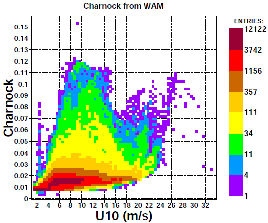
\includegraphics{FIG_wave/WAM_Charnock.png}}\par
\end{minipage}
\begin{minipage}{5.3cm}
\centering
\resizebox{5.5cm}{!}{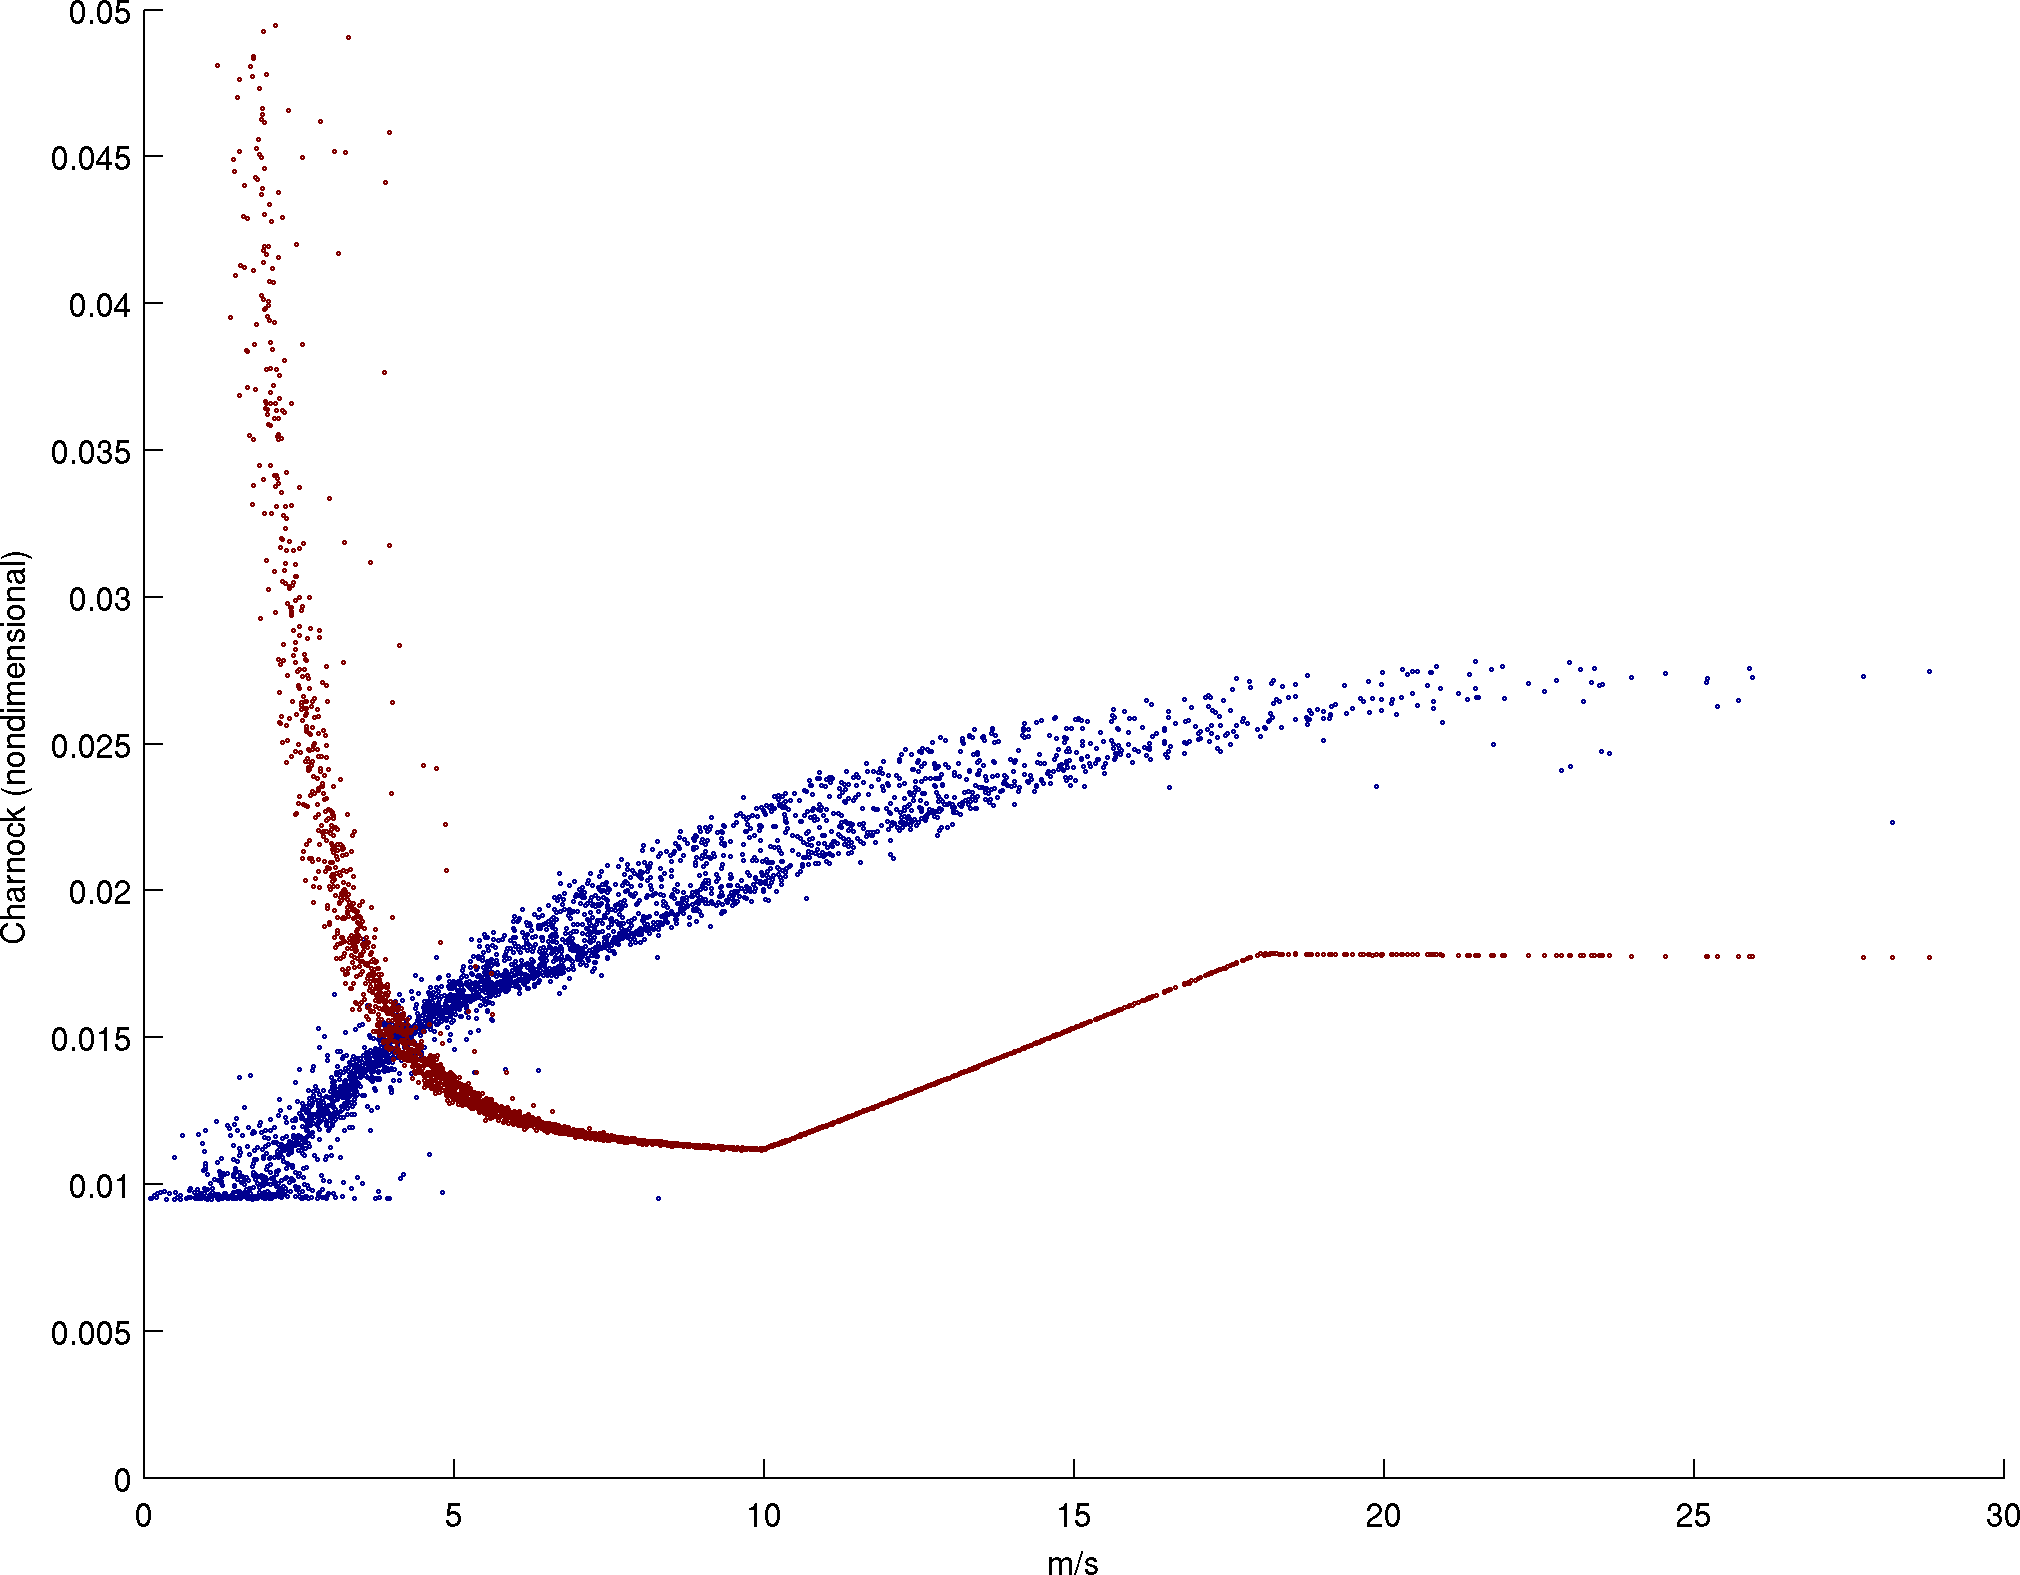
\includegraphics{DrifterPicture/Scatter_Charnock/Scatter_bulk_wave.png}}\par
\end{minipage}
\end{center}

\begin{itemize}
\item There are large variability of Charnock expressed in function of the wind.
\item A priori, the wave model has a good idea of the roughness of the sea and so it makes sense to use the Charnock coefficient computed from the wave model.
\end{itemize}
}

\frame{
  \frametitle{Coupling of {\tt WAM} and {\tt COSMO}}
\begin{itemize}
\item Both models were coupled with the {\tt PGMCL}.
\item We follow the same strategy as the one between {\tt IFS} and {\tt WAM}.
\begin{center}
\resizebox{4cm}{!}{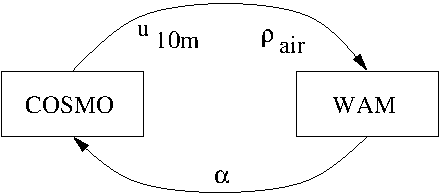
\includegraphics{FIG_wave/Model_CouplingWAM_COSMO.pdf}}\par
\end{center}
\item We run the model over a period of two months over the Mediterranean Sea for Nov. Dec. 2010
\begin{center}
\resizebox{4cm}{!}{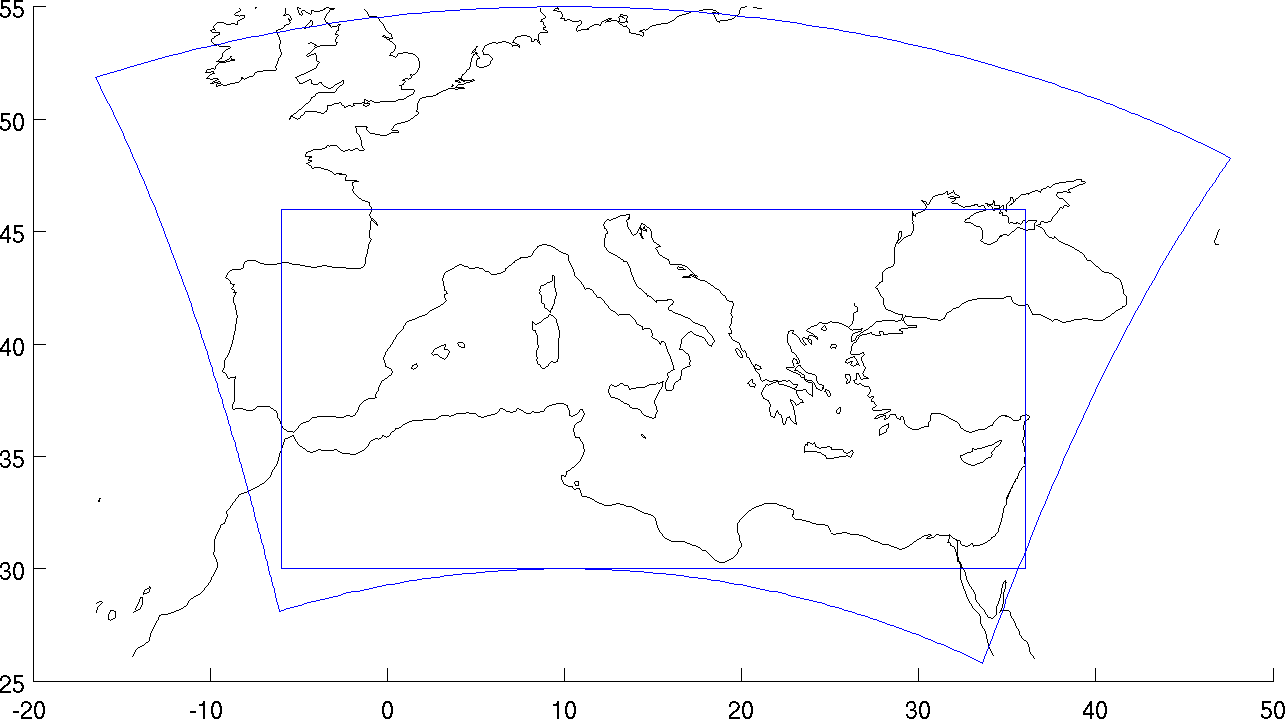
\includegraphics{FIG_wave/MapSimulation.png}}\par
\end{center}
\end{itemize}
Work done in collaboration with P. Janssen/J. Bidlot ({\tt ECMWF}), L. Cavaleri ({\tt ISMAR}), L. Torrisi ({\tt CNMCA}, Italian Nat. Met. Center) and A. Roland (TU Darmstadt)
}


\frame{
  \frametitle{Wave height comparison (ENVISAT altimeter)}

\begin{center}
\begin{minipage}{5.3cm}
\centering
\resizebox{5.5cm}{!}{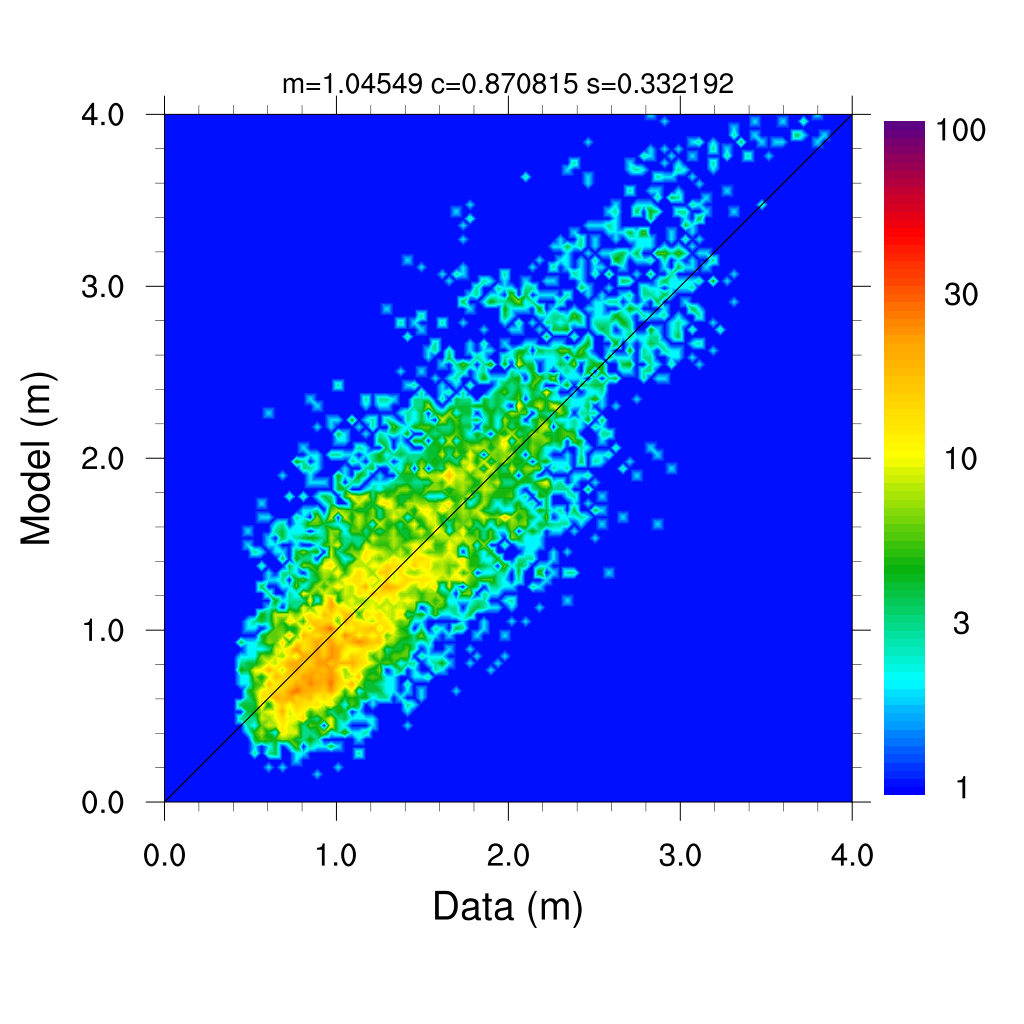
\includegraphics{COSMOWAM/RUN_coupled/AltimeterStat/Scatter_ENVISAT_Wave.png}}\par
Coupled
\end{minipage}
\begin{minipage}{5.3cm}
\centering
\resizebox{5.5cm}{!}{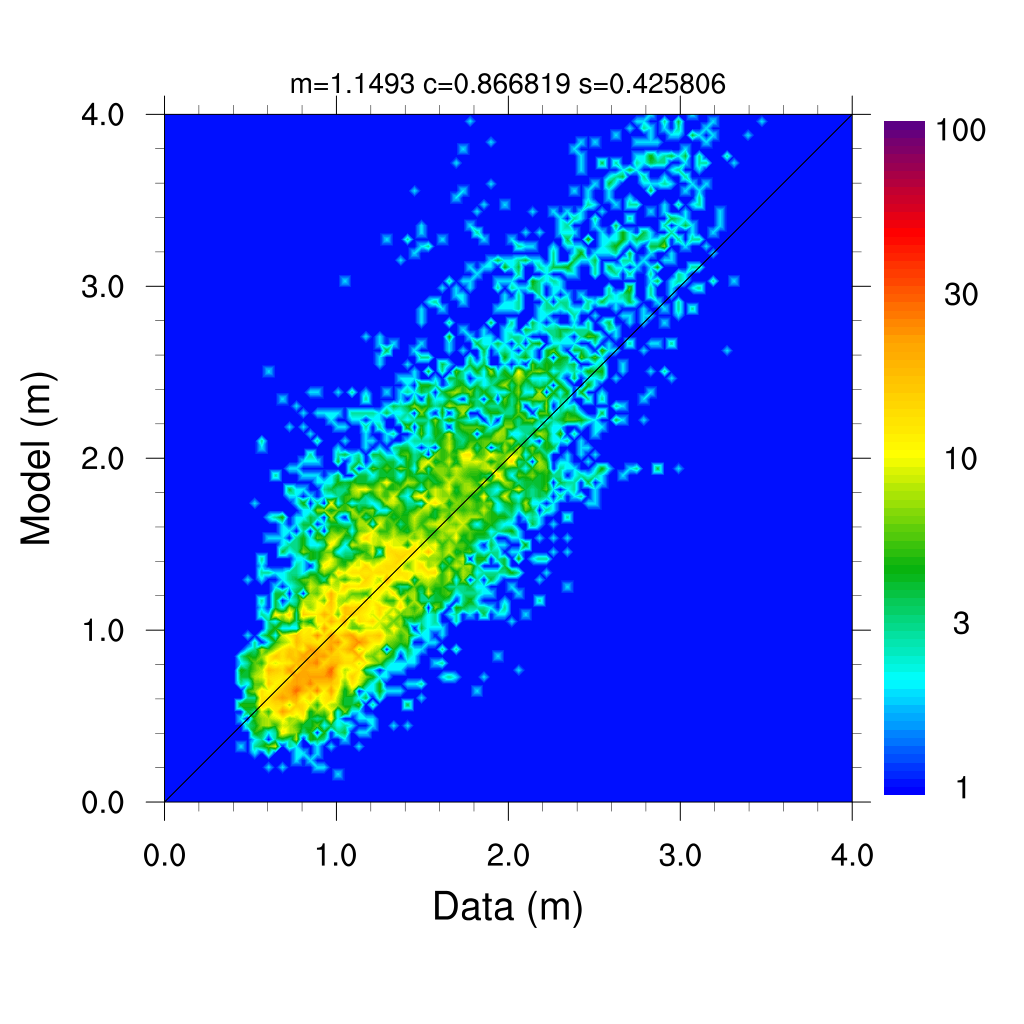
\includegraphics{COSMOWAM/RUN_uncoupled/AltimeterStat/Scatter_ENVISAT_Wave.png}}\par
Uncoupled
\end{minipage}
\end{center}
}


\frame{
  \frametitle{Wind speed comparison (ENVISAT altimeter)}

\begin{center}
\begin{minipage}{5.3cm}
\centering
\resizebox{5.5cm}{!}{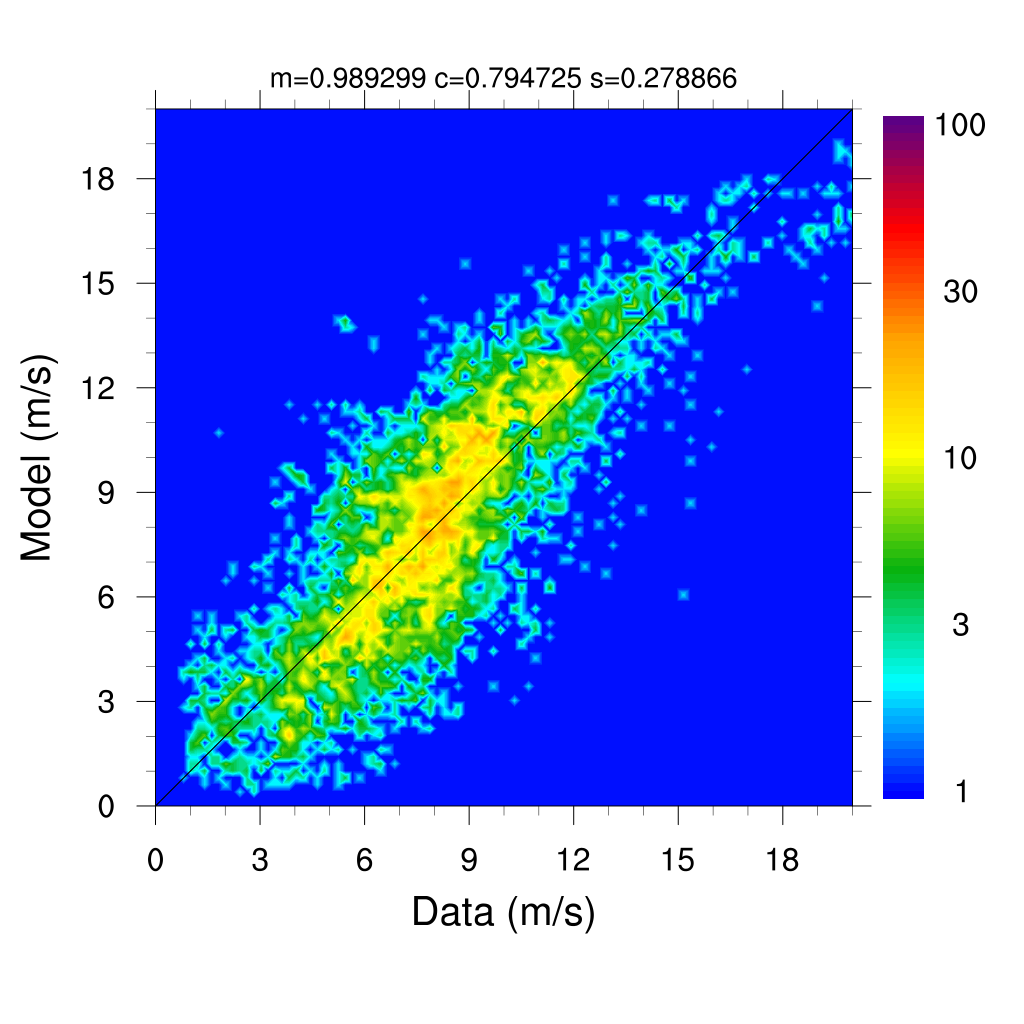
\includegraphics{COSMOWAM/RUN_coupled/AltimeterStat/Scatter_ENVISAT_Wind.png}}\par
Coupled
\end{minipage}
\begin{minipage}{5.3cm}
\centering
\resizebox{5.5cm}{!}{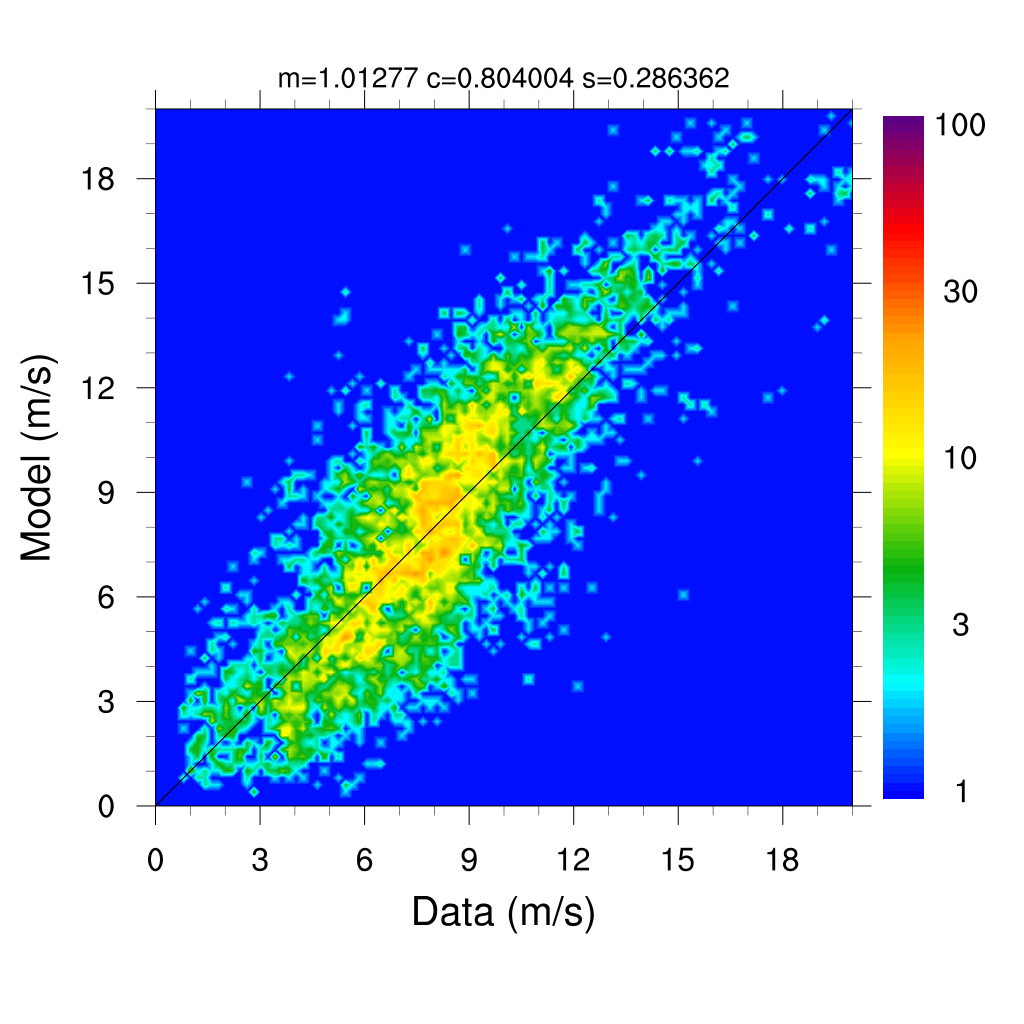
\includegraphics{COSMOWAM/RUN_uncoupled/AltimeterStat/Scatter_ENVISAT_Wind.png}}\par
Uncoupled
\end{minipage}
\end{center}
}



\frame{
  \frametitle{Triple coupling}

\begin{itemize}
\item We also designed a system where we can do the coupling of all models together:
\begin{itemize}
\item Circulation: ROMS
\item Atmosphere: COSMO
\item Wave: WWM or WAM in structured or unstructured
\end{itemize}
\item The coupling Wave-Atmosphere and Wave-Circulation is done as before.
\item The coupling Ocean-Atmosphere is done in following way:
\begin{itemize}
\item The atmospheric model provides Wind, Air Pressure, humidity, short/long radiation to the model.
\item The circulation model provides Sea Surface Temperature to the atmosphere
\end{itemize}
\item The setting is modular and models can be added as wished.
\end{itemize}
}



%\frame{
%  \frametitle{Results}
%ME: Mean Error \mbox{~~~~} RMSE: Root Mean Square Error
%\begin{itemize}
%\item For comparison of wave height with all buoys we get:
%\begin{center}
%\begin{tabular}{|c|c|c|}
%\hline
%         & ME     & RMSE\\
%\hline
%Coupled     & 0.11 m & 0.55 m\\
%Uncoupled   & 0.21 m & 0.62 m\\
%\hline
%\end{tabular}
%\end{center}
%\item For comparison of wave height with Envisat altimeter satellite we get:
%\begin{center}
%\begin{tabular}{|c|c|c|}
%\hline
%         & ME    & RMSE\\
%\hline
%Coupled     & 0.25 m  & 0.65 m\\
%Uncoupled   & 0.43 m  & 0.85 m\\
%\hline
%\end{tabular}
%\end{center}
%\item For comparison of wind speed at $10$m with Envisat altimeter satellite we get:
%\begin{center}
%\begin{tabular}{|c|c|c|}
%\hline
%         & ME       & RMSE\\
%\hline
%Coupled     & 0.25 m/s & 2.28 m/s\\
%Uncoupled   & 0.44 m/s & 2.44 m/s\\
%\hline
%\end{tabular}
%\end{center}
%\end{itemize}
%}







%\frame{
%  \frametitle{Grids of the Adriatic}
%trim=l b r t
%\begin{center}
%\begin{minipage}{5.2cm}
%\resizebox{5.2cm}{!}{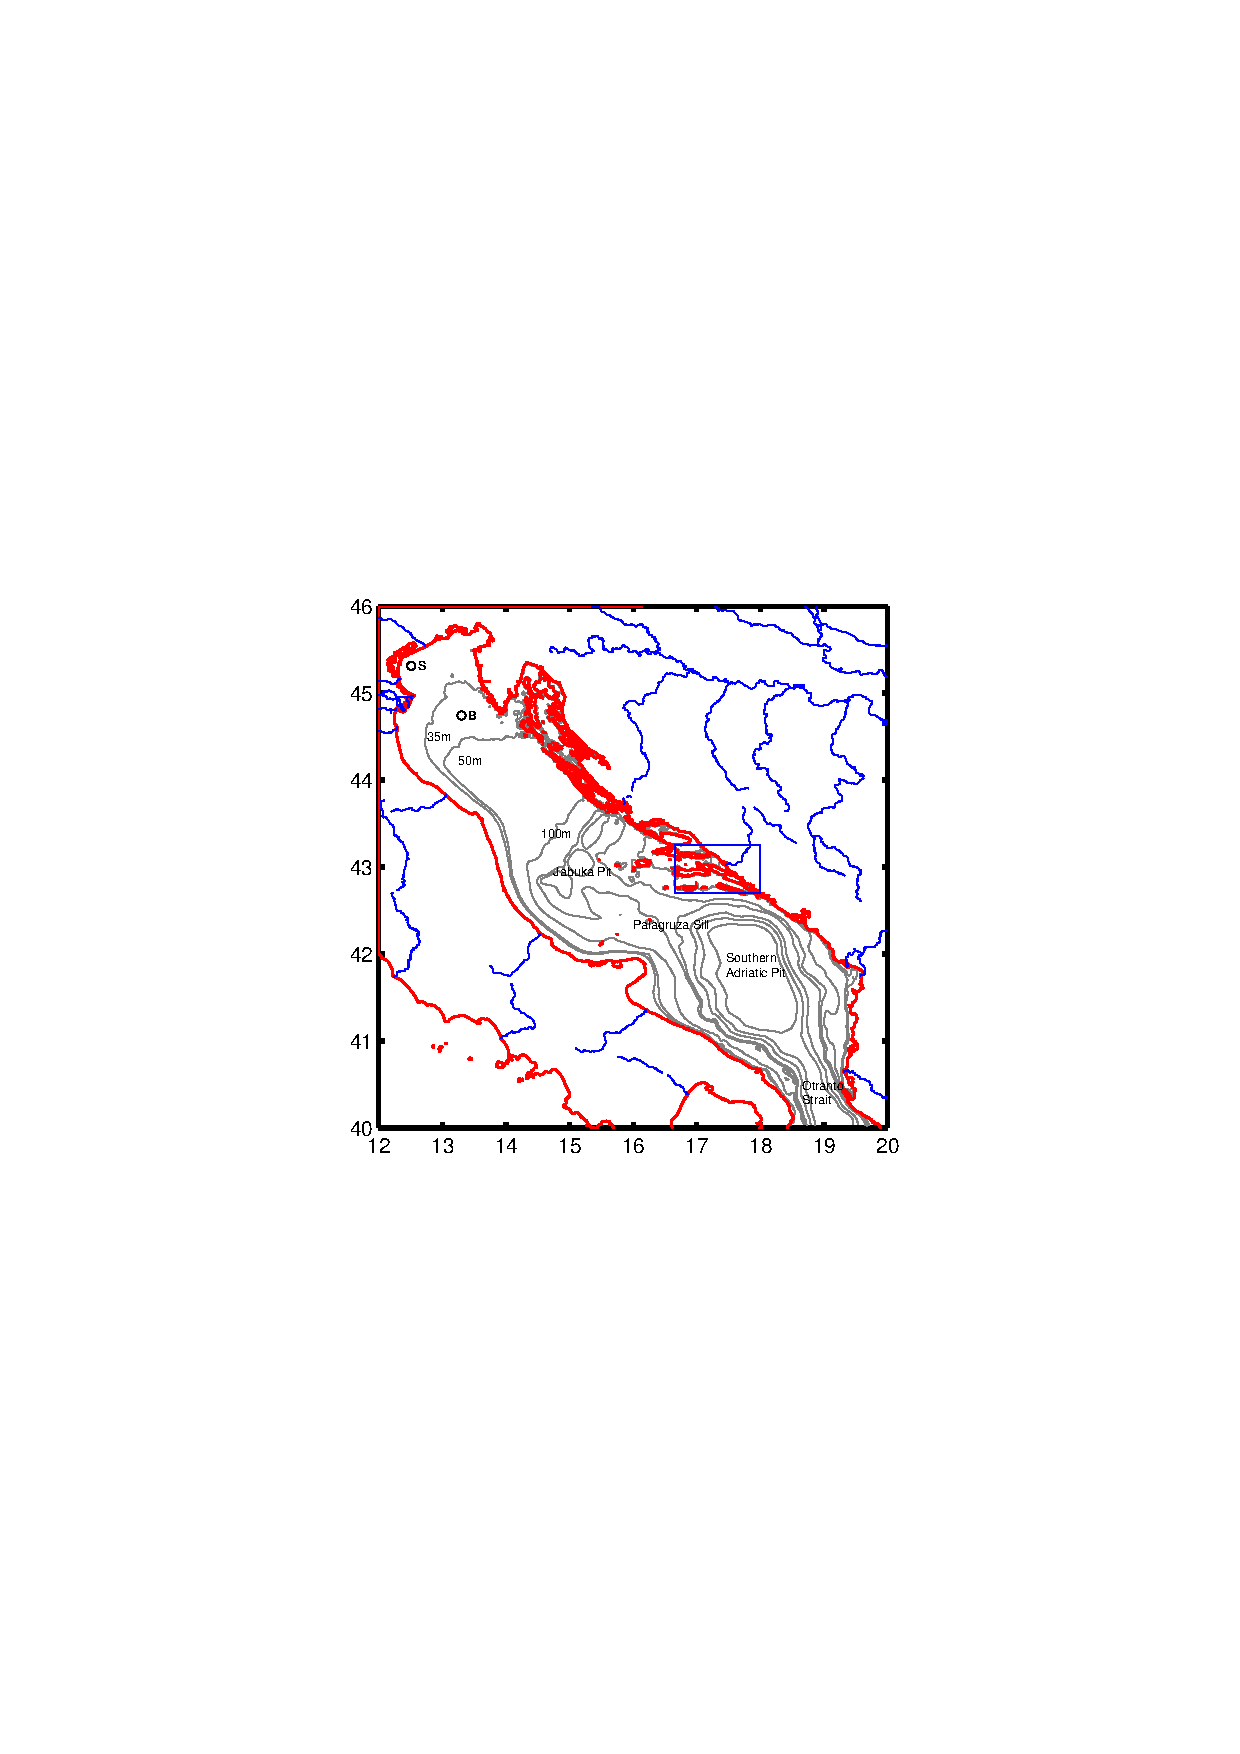
\includegraphics[bb=166 390 399 555,clip]{FIG_wave/Stations300_AASSb.pdf}}\par
%\end{minipage}
%\begin{minipage}{5.2cm}
%\resizebox{6.3cm}{!}{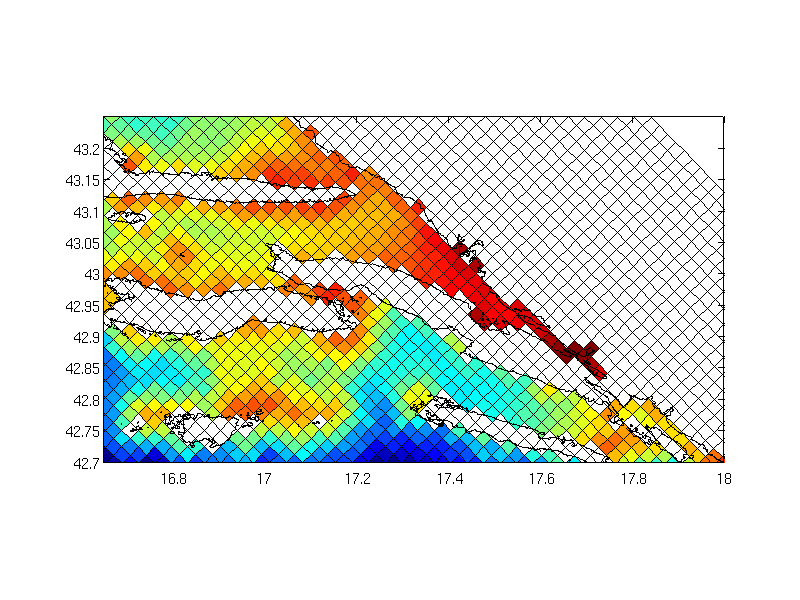
\includegraphics[trim=16mm 28mm 16mm 28mm, clip]{FIG_wave/PicCompar/RomsGrid.png}}\par
%\end{minipage}
%\end{center}
%\begin{center}
%\begin{minipage}{5.2cm}
%\resizebox{5.8cm}{!}{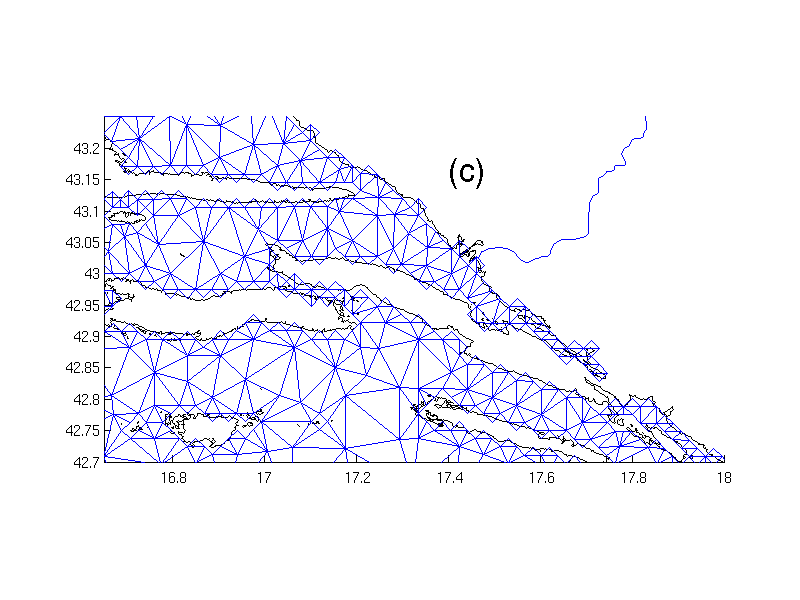
\includegraphics[trim=16mm 28mm 16mm 28mm, clip]{FIG_wave/PicCompar/FEMgrid1.png}}\par
%\end{minipage}
%\begin{minipage}{5.2cm}
%\resizebox{5.8cm}{!}{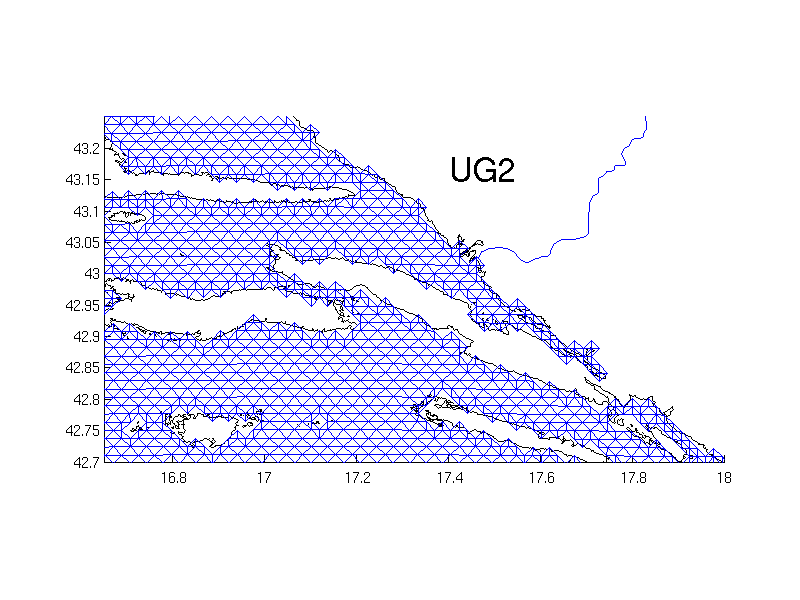
\includegraphics[trim=16mm 28mm 16mm 28mm, clip]{FIG_wave/PicCompar/FEMgrid2.png}}\par
%\end{minipage}
%\end{center}
%}






\end{document}
